\documentclass{article}
\usepackage{amsmath,splitbib,epsfig,times,program,multicol,amsfonts}

\setlength{\textheight}{9.0in}
\setlength{\columnsep}{0.25in}
\setlength{\textwidth}{6.75in}
\setlength{\topmargin}{-0.25in}
\setlength{\headheight}{0.0in}
\setlength{\headsep}{0.0in}
\setlength{\evensidemargin}{-0.125in}
\setlength{\oddsidemargin}{-0.125in}
\sfvariables
\normalbaroutside

\makeatletter
\newenvironment{tablehere}
  {\def\@captype{table}}
  {}

\newenvironment{figurehere}
  {\def\@captype{figure}}
  {}
\makeatother

\DeclareMathOperator{\READ}{R}
\DeclareMathOperator{\WRITE}{W}
\DeclareMathOperator{\IsRace}{IsRace}

\begin{category}[A]{Dynamic Analysis for Verification}
  \SBentries{694486,964023,940116,havelund00using,265927,wang03runtimeRV,512560,302467,karaorman99jcontractor}
\end{category}
\begin{category}[B]{Model Checking Software}
  \SBentries{Robby-etal:TACAS2004,yang04using,775928,776863,henzinger03software,musuvathi:osdi:cmc,ball01automatic,786967,corbett00language,ball00bebop,263717}
\end{category}
\begin{category}[C]{Extended Static Analysis}
  \SBentries{DBLP:conf/ecoop/2004,512558,512538,349332,tkachuk03automated,hovemeyer04finding,1007543,195297,231389,zitser04testing}
\end{category}

\begin{document}
\title{Approaches to Program Checking}
\author{Graham Hughes}
\date\today
\maketitle

\begin{multicols}{2}

% Stuff to do before presentation: make sure I understand the scalable
% flow analysis better

\section{Introduction}

Automatically checking programs for errors has long been a frustrated
dream.  The increasing size, widespread use of concurrency, and new
visibility of security problems has given an impetus to this broad
discipline.  Many new algorithms and tools for finding errors have
been created including the important category of model checkers
designed to run on real programs.

In this report I will survey three classes of program analysis
techniques:
\begin{itemize}
\item \textit{Dynamic analysis for verification}, which is to say
  dynamic monitoring of a running program for the purpose of verifying
  that certain properties are upheld;
\item \textit{Extended static analysis}, which encompasses a field of
  analysis tools attempting to prove important properties of programs
  without running them;
\item and \textit{Model checking software}, which tackles the tricky
  problem of systematically exploring all behaviors of real code.
\end{itemize}
There is extensive cross pollination between these fields and I would
be amiss in not mentioning the cross references; accordingly many of
the paper summaries will refer to one another.

Following this survey, I will discuss some work I did during an
internship at Fujitsu, where I succeeded in discovering several errors
in a commercial project using a model checker.

Since many of these programs are very different and measure different
things, it's not really possible to have one consistent example.  I
reuse them as much as is possible and will refer to preexisting
figures as needed.

\section{Dynamic Analysis for Verification}

The goal in a dynamic analysis is to instrument a program to keep
track of ``events''---the exact nature of which depends on the
analysis---and then run the program normally.  This has several
advantages: it tends to be relatively easy to implement, it can lead
to some very precise results, and the analysis can usually possess
precise knowledge of the control flow.  The main disadvantage is that
the analysis these tools can give is limited by the execution run; if
a situation only occurs on certain execution paths and the test suite
used to drive the program does not exercise them, then the analysis
tools may not be able to detect the problem.

Dynamic analysis is frequently best suited to verifying global
properties of a program that are not amenable to local analysis and
where the execution path sensitivity of the run can be controlled.
The old standby here was manual memory allocation in C, an inherently
global property of a system that was notoriously difficult for
programmers to control.  Today, with the recent explosion of interest
in concurrent programs and the associated concurrency problems of race
conditions and deadlock, several dynamic analysis tools explore that
space.

I will use the Eraser paper to describe these tools in detail because
in some ways it epitomizes the best dynamic analysis: it is not
particularly sensitive to the execution path of the program; it is
very useful; it looks for global properties of a system that can arise
from modules that are locally correct being combined inappropriately;
and it is useful in connection with other techniques, most notably
driving a model checker as described in~\cite{havelund00using} of
which I will speak later.

\subsection{Eraser~\cite{265927}}

Eraser instruments C programs to provide dynamic detection of data
races, specifically in the context of lock-based synchronization.  In
this framework, races can occur if all of the following conditions
hold: two different threads access the same shared variable, one of
the accesses is a write, and there is no explicit mechanism to prevent
concurrent modifications.  In the context of lock-based
synchronization, this means that, a race can happen if the two threads
accessing the same variable hold no locks in common at the time of the
access.

Previous efforts toward this sort of detection used a technique based
on happens-before analysis; that technique can accommodate any sort of
synchronization, but it is slow and path dependent.  Eraser's use of
lock-based synchronization makes this much easier.

Eraser implements the LockSet algorithm.  A first stab at an algorithm
like this might be built around the idea is that every shared variable
should be protected by some lock, and that the algorithm will monitor
all reads and writes and infer the manner in which the variable is
protected from the execution history.  Thus, for each variable $v$,
$C(v)$ is the set of candidate locks for $v$---that is, all locks that
have protected $v$ for the computation so far.  Initially this is all
locks, and at each read/write if $L$ is the set of locks held by the
current thread, $C(v)$ is updated to $C(v) \cap L$.  Then, if $C(v)$
ever becomes empty, no lock consistently protects accesses to $v$ and
a warning is issued.

This turns out to be too strict, for several reasons.  First, shared
variables are frequently initialized without any locks being held.
Second, some shared variables are initialized and after that are only
read, which is not dangerous.  Finally, holding a read/write lock in
read mode does not make writes safe.  To accommodate the first
concern, Eraser associates a state in a state machine with each shared
variable.  The state machine is shown in Figure~\ref{fig:eraser}.

\begin{figure*}
  \begin{center}
    \leavevmode
    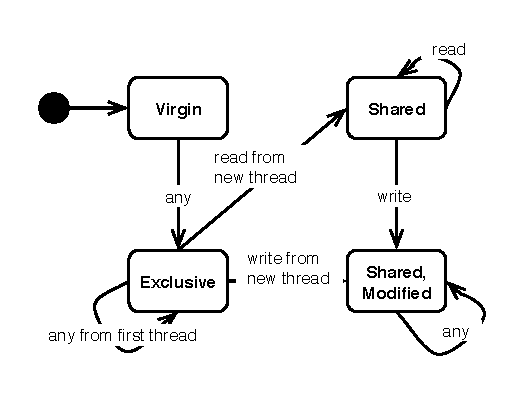
\includegraphics{eraser}
  \end{center}
  \caption{LockSet state machine}
  \label{fig:eraser}
\end{figure*}

Warnings are only issued in the shared-modified state.  This makes the
algorithm slightly dependent on the exact path that was taken through
the system, certainly more so than would be preferable.  However, this
doesn't appear to have been a problem in practice.

To handle read/write locks, the authors modify their criteria
slightly, so that for a thread $t$ on a read event $C(v) \leftarrow
C(v) \cap LocksHeld (t)$ and on a write event $C(v) \leftarrow C(v)
\cap WriteLocksHeld (t)$---this way, locks in read mode are removed
when a write occurs.

Finally, to handle some of the various classes of false alarms that
come up, there are numerous function calls that are essentially
annotations.  The major things that Eraser cannot handle by default
are memory pools (to avoid malloc/free costs for specialized types of
memory objects) and private synchronization primitives; also an
ignore-warnings annotation for ignoring benign races.  These are
uninteresting in a theoretical sense but essential to make the tool
useful in a practical sense.

To test their implementation the authors ran it on the AltaVista
search program, a cache server for a software configuration management
system, and a distributed storage system.  They found several races,
some serious, in all of these.  A small number of annotations sufficed
to silence the false alarms; the others represented some serious
issues.

\subsection{Concurrency}

A few other interesting dynamic concurrency tools are:

\subsubsection{Atomizer, a Dynamic Atomicity Checker~\cite{964023}}

An interesting development in concurrency analysis is that the
standard race detection algorithms aren't always sufficient.  The
example this paper cites is from the Java standard libraries, but a
smaller example is in Figure~\ref{fig:atomicfail}.  The characteristic
of interest is this: correlations expected between times that an
object is locked (for example, calling two different synchronized
methods on a Java object) may be broken.  As an alternate model, the
authors propose \textit{atomicity}, which is a property of a block of
code.

Figure~\ref{fig:atomicfail} can be modified to be atomic and sound,
yet not race free; this is shown in Figure~\ref{fig:atomicsuccess}.
Both these examples are taken from Flanagan's presentation to PADTAD
2004.

\begin{figure*}
  \hfill
  \begin{minipage}[t]{.45\textwidth}
    \begin{center}
      \begin{small}
\begin{verbatim}
class Account {
  private int balance = 0;
  public synchronized int read () {
    return balance;
  }
  public void deposit (int n) {
    int r = read ();
    synchronized (this) {
      balance = r + n;
    }
  }
}
\end{verbatim}
      \end{small}
      \caption{A program that is not atomic but race free}
      \label{fig:atomicfail}
    \end{center}
  \end{minipage}
  \hfill
  \begin{minipage}[t]{.45\textwidth}
    \begin{center}
      \begin{small}
\begin{verbatim}
class Account {
  private int balance = 0;
  public int read () {
    return balance;
  }
  public void deposit (int n) {
    synchronized (this) {
      int j = balance;
      balance = j + n;
    }
  }
}
\end{verbatim}
        \caption{A program that is not race free but is atomic (and safe)}
        \label{fig:atomicsuccess}
      \end{small}
    \end{center}
  \end{minipage}
  \hfill
\end{figure*}

In more detail, the goal is that any execution of atomic blocks is
equivalent to some serialized execution---that is, if atomic blocks
$a$ and $b$ are running concurrently, any execution where bits of $a$
and $b$ are interleaved is equivalent to either the execution $a;b$
or the execution $b;a$.  This reduces the problem of understanding
the concurrent program in general to understanding some serial
interleaving of that same program, something much easier.  Several
interleaved executions are shown in Figure~\ref{fig:blockmoving}.

One way to determine that a block is atomic is to use reduction.  To
explain this, I fix $a$ and $b$ as blocks of code, which comprise
several statements I denote $a_1, a_2, \dots, a_n$ and $b_1, b_2,
\dots, b_m$ respectively.  These statements should be indivisible; for
example, perhaps they are Java byte codes.  Then, one particular
concurrent execution might be $a_1 b_1 b_2 a_2 \dots b_{m-1} b_m
a_{n-1} a_n$.

We divide statements into four categories: right movers, left movers,
both movers, and non movers.  Right movers are statements with the
property that if $x_i$ is a right mover and $y_j$ is any statement
from another thread, then the interleaved execution $\dots x_i y_j
\dots$ is equivalent to $\dots y_j x_i \dots$.  Rephrasing, right
movers commute to the right with any statement from any other thread.
Similarly, left movers commute to the left, both movers are left
movers and right movers, and non movers are any other statement.  As
examples of each category, we can note that lock acquisition is a
right mover; that lock release is a left mover; that access to a
protected variable is a both mover; and that an access to an
unprotected variable is a non-mover.  Figure~\ref{fig:blockmoving}
also describes the reduction process, where an interleaved execution
can be demonstrated to be equivalent to a serial execution.

\begin{figure*}
  \begin{center}
    \leavevmode
    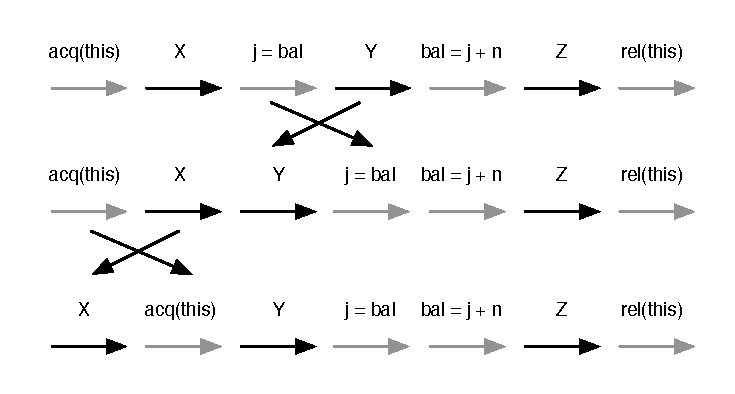
\includegraphics{reduction}
  \end{center}
  \caption{Reduction equivalence}
  \label{fig:blockmoving}
\end{figure*}

Given this framework, any block of code that satisfies the ``regular
pattern'' $(R + B)* N? (L + B)*$ (that is, the block begins with any
number of right or both movers, may contain a non-mover, and ends with
any number of left or both movers) is atomic.  This is a sufficient
but not necessary condition for atomicity.

Atomizer the tool attempts to prove that blocks are atomic during
execution by instrumenting the program, attaching a binary state to
every alleged atomic block.  When execution in such a block begins,
the block is in the InRight state.  Any statements that are right
movers do not change the state.  Access to variables is checked---if
the access is protected, then it's a both mover and the state doesn't
change; otherwise it's a non mover and the block state transitions
into the InLeft state.  Similarly, left movers and any other singular
non mover will also cause this transition.  After this, any right
movers or non movers seen before the block ends are a violation of the
atomicity property.

Atomizer needs to know the set of locks that protect each variable,
and it uses the LockSet algorithm from Eraser to do this.  This does
mean that variable accesses can be inappropriately tagged as both
movers before the tool figures out how the locks really work.  This is
suboptimal but hard to avoid and the authors make no real effort to
correct for it.  Since any such access would also show up running
Eraser, running Eraser first, correcting any claimed races, and then
running Atomizer to verify atomicity properties should be sufficient.

An additional issue is the determining of what is and is not an atomic
method.  One can annotate a block as declaring one in Atomizer, but it
also uses a simple heuristic, assuming that all synchronized blocks
and all public methods except for \texttt{main} and \texttt{run} are
supposed to be atomic.

\subsubsection{Efficient and Precise Datarace Detection~\cite{512560}}

This paper describes a run time data race detector that is different
from Eraser.  The new algorithm is fast without sacrificing precision.
To explain the algorithm, let us give some definitions.  We are mostly
interested in memory events here, so define an event as a five tuple
$(t, L, m, a, x)$, where $t$ is the thread where the event occurs, $L$
is the set of locks held by that thread, and $m$ is the ``location''
of the event, $a$ is $\READ$ or $\WRITE$ depending on whether a read
or a write occurred, and $x$ is some bookkeeping information that we
do not further consider.  I refer to the first component of an event
$e$ as $e.t$, and similarly for the other parts.

We need a few more definitions still.  The authors define a meet
operation on accesses, where we define $\READ \sqcup \READ = \READ$
and $\WRITE \sqcup \, x = \WRITE$.  We also need a join operation for
threads; for threads $t_i, t_j$, the authors require that $t_i \sqcap
t_i = t_i$, $t_i \sqcap t_\top = t_\top \sqcap t_i = t_i$ and $t_i
\sqcap t_j = t_\bot$ if $i \neq j$.

Then, we may declare that two events $e_i, e_j$ are a race if they
access the same memory location in different threads with no common
locks and one of them being a write: that is,
\begin{multline*}
\IsRace(e_i, e_j) \equiv e_i.m =
e_j.m \wedge e_i.t \sqcap e_j.t = t_\bot \wedge \\ e_i.L \cap e_j.L = \emptyset
\wedge e_i.a \sqcup e_j.a = \WRITE
\end{multline*}

The set of all racy accesses could be as big as $O(N^2)$ for $N$
accesses.  We are not interested in all of them, and so look to reduce
the set.  The authors note that given events $e_i, e_j$, we don't need
to consider $e_j$ at all if for all future events $e_k$ $\IsRace (e_j,
e_k) \rightarrow \IsRace (e_i, e_k)$.  If this condition holds, we say
that $e_i$ is weaker than $e_j$.  Using this condition we can tame the
size of the race set, at the cost of enumerating all races.  The new
algorithm does guarantee that one race for every memory location that
has one will be generated.

To collect this data at run time, the paper describes a trie-based
algorithm.  For each memory location there is a trie, and the edges of
that trie are ids of lock objects; the nodes hold thread and access
type information for the set of events there.  Multiple thread ids are
not stored, only the join according to $\sqcap$.  Similarly, only the
meet of the access events is stored; so it is $\READ$ if every access
has been a read, or $\WRITE$ otherwise.

Given this, if we encounter a new event $e$ we first walk the trie
following links that are in $e.L$.  If any encountered node is weaker
than $e$, discard $e$.  Otherwise, we must check $e$ for races using a
recursive traversal of the trie.  For every node $n$, if the last edge
followed is in $e.L$, then $n$ and any accesses below it cannot
possibly be a race; prune the search here.  Otherwise if $n.t \sqcap
e.t = t_\bot$ and $n.a \sqcup e.a = \WRITE$, then there is a
legitimate race here; it should be reported immediately and traversal
terminated.  Finally, if neither of the previous two conditions hold,
we should recursively traverse $n$'s children.

If we can run through the above steps without incident, then any node
whose path to the root is labeled using elements of $e.L$ should be
updated; for each such node $n$, set $n.t \leftarrow n.t \sqcap e.t$
and $n.a \leftarrow n.a \sqcap e.a$.  If no nodes like this are found,
then a new one for $e$ should be added; the trie will need to be
walked again to remove anything stronger than the new node.

This approach involves a lot of trie traversals.  There are some
optimizations discussed in the paper involving event caches and some
static analysis techniques to rule out any accesses that cannot cause
races.  As well, there is another optimization during the
instrumentation phase, where a static weaker-than relation is used to
avoid inserting unnecessary instrumentation.

\subsubsection{Run-Time Analysis for Atomicity~\cite{wang03runtimeRV}}

Like Atomizer~\cite{964023}, this paper describes a dynamic algorithm
to determine the atomicity properties of a program.  This paper first
describes the reduction analysis that Atomizer uses.  This paper
concludes that reduction is useful but too simple; there are many
atomic methods that cannot be proven to be atomic using pure
reduction.  Accordingly the authors describe a more expensive block
based algorithm that is precise but has exponential run time.

Simply put, the algorithm is computes all feasible interleavings and
then checks them for things that are definitely not atomic.  It is
defined using a series of algorithms, each more general than the last;
the penultimate algorithm checks problems between a pair of threads,
and the ultimate one checks all pairs.

This general problem is, like many other interesting problems, NP
complete.  As a result, reduction analysis is much more useful, and
research has gone into extending reduction with techniques like
purity.  This last step is done in~\cite{1007543} which is described
later.

\subsection{Safety}

A popular application for dynamic analysis is keeping track of a
running program and making sure that it hasn't violated some
fundamental properties that should be upheld.

\subsubsection{jContractor~\cite{karaorman99jcontractor}}

A proposed discipline for writing good programs is Design By
Contract\cite{meyer92applying}, sometimes abbreviated DbC.  Design By
Contract has a number of design related implications, but among the
more direct propositions is that methods should check that their input
arguments are valid and that they are generating appropriate output.
The language Eiffel~\cite{meyer92eiffel} contains constructs to
support this technique, but Java does not.

jContractor attempts to introduce Design By Contract principles into
Java, and to enforce them when applicable.  The constructs that are
enforced include Eiffel-style method preconditions, postconditions and
object invariants.  jContractor's architecture is such that these
techniques are integrated into the Java program on a byte code level,
permitting the use of standard Java compilers and JVMs.  There exist
other DbC tools for Java, but they tend to work through stylized
comments and sometimes cannot handle interfaces.  An example of the
latter is the Jass~\cite{detlef99jass} tool.

Given a method---perhaps named ``\texttt{int} \texttt{add}
\texttt{(Item i)}'' in a WorkList class---to introduce a precondition
using jContractor, one writes a new method in the WorkList class named
\texttt{boolean add\_PreCondition (Item i)}.  Here the argument list
is that of the original method and this new method is expected to
return true or false depending on whether the precondition is
satisfied or unsatisfied.  Similarly, to introduce a postcondition one
writes a new method \texttt{boolean} \texttt{add\_PostCondition}
\texttt{(Item i)} with an argument list the same as that of the
original method and which can compare a value to the return value of
the method using the syntax \texttt{RESULT.compare} $(expr)$.  The
postcondition can also get access to the original object before the
method was invoked using \texttt{OLD}.  In a similar fashion, the
invariant for the entire object is in the method \texttt{boolean}
\texttt{WorkList\_ClassInvariant} \texttt{()}, and is checked on entry
and exit of any method on an instrumented class.  There also exist
additional patterns for special behavior when the method throws an
exception.

The idea behind the approach is that the Java compiler will handle
turning these methods into Java byte code automatically; all that is
necessary to fold these into the normal Java execution is that a
special class loader be used.  This special loader will look for
methods named in the above fashion and insert them into the
instrumented method in the appropriate place, at class load time.
Through a special alternate mechanism, contracts can be added to
classes for which the source is unavailable, and also interfaces.

Inheritance needs to be dealt with; since for any given Java class any
of its superclasses as well as any interfaces it implements can have
contracts, the algorithm needs to deal with multiple inheritance.
JML\cite{burdy03overview}, a modeling language for Java, describes an
robust lattice based algorithm for handling this.  jContractor simply
takes the conjunction of all preconditions and the disjunction of all
postconditions, with some important heuristics to ensure that a
programmer does not inadvertently write code believing that he can
narrow a precondition or widen a postcondition.

\subsubsection{Monitoring a Running Program~\cite{694486}}

Here, the goal is to test properties of an executing program.  The
program is instrumented so that it sends events to a separate monitor
program, which ensures that these events do not represent a violation
of some user-specified safety properties.  These properties are
expressed in a new temporal logic ``past time LTL'' or ptLTL.  A ptLTL
formula can be translated into a program that can check a finite trace
of events in time linear to the size of the trace while using constant
memory.

ptLTL is similar to normal LTL, but all the primitives speak of events
that have occurred, never events that will occur.  The version of
ptLTL that is used in this paper contains several logically redundant
operators that are nonetheless useful for expressing important
properties.  Also, the size of generated code is dependent on the
ptLTL expression, and using powerful operators makes for faster
analysis.  An example formula is something like $ \uparrow p
\rightarrow [ q, \downarrow (r \vee s))_s$; that formula encodes the
condition ``if $p$ is true, then $q$ has been true in the lifetime of
the execution trace, and since $q$ was true $r \vee s$ has been
true.''

Evaluating such a formula can be done through a fairly straightforward
application of dynamic programming.  The first step is to enumerate
the formula, so that the number of any part of the formula is smaller
than all of its subformulae.  The formula's behavior can be described
in a matrix $s[1 \dots n, 0 \dots m]$ of Boolean values, where $n$ is
the number of data sets collected, $m$ is the maximal enumeration
number in the formula, and $s[i, j]$ is the truth value of the
subformula numbered $j$ after the $i$th data set has been analyzed.
In the above example $m$ is 8.

The above suggests that we store all data sets in memory, but in fact
we only need $s[i, 0 \dots m]$ and $s[i - 1, 0 \dots 8]$ due to the
way the past time LTL operators are defined.  Then, if we rename $s[i,
0 \dots m]$ to $now[0 \dots m]$ and rename $s[i - 1, 0 \dots m]$ to
$pre[0 \dots m]$, we can compute $now[i]$ using the current state of
any predicates (in the example, $p$, $q$, $r$, $s$), $now[i+1 \dots
m]$ and $pre[0 \dots m]$.  Here, I show a translation of the example
formula above which was taken from the paper.  In that example, \(
|state| \) is something that the predicates $p$, $q$, $r$ and $s$ use
to determine whether to return true or false.
\begin{program}
  \FUNCT |check|(t = e_1 e_2 \dots e_n) \BODY
  \EXP |state| := \emptyset;
  |pre|[0..8] := (|false|, |false|, \dots, |false|);
  |now|[0..8] := (|false|, |false|, \dots, |false|);
  |state| := |update| (|state|, e_1);
  |pre|[8] := s(|state|);
  |pre|[7] := r(|state|);
  |pre|[6] := |pre|[7] \vee |pre|[8];
  |pre|[5] := |false|;
  |pre|[4] := q(|state|);
  |pre|[3] := |pre|[4] \wedge \neg |pre|[5];
  |pre|[2] := p(|state|);
  |pre|[1] := |false|;
  |pre|[0] := \neg |pre|[1] \vee |pre|[3];
  \FOR i := 2 \TO n \STEP 1 \DO
  |state| := |update| (|state|, e_i);
  |pre|[8] := s(|state|);
  |pre|[7] := r(|state|);
  |pre|[6] := |now|[7] \vee |now|[8];
  |pre|[5] := \neg |now|[6] \wedge |pre|[6];
  |pre|[4] := q(|state|);
  |pre|[3] := (|pre|[3] \vee |now|[4]) \wedge \neg |pre|[5];
  |pre|[2] := p(|state|);
  |pre|[1] := |now|[2] \wedge \neg |pre|[2];
  |pre|[0] := \neg |now|[1] \vee |now|[3];
  \IF |now|[0] = |false|
  \THEN |error| (``property violated'');
  \FI;
  |pre| := |now|
  \OD \ENDEXP \ENDFUNCT
\end{program}

There are several optimizations possible---for example, the past value
of every value of every subformula is probably not necessary.  Also,
the function calls for state properties are the most expensive current
component; if they could be encoded as binary decision diagrams
(abbreviated BDDs), then they could be inserted inline using the ?:
operator: so if $p \equiv x == 4 \vee y < x$, it could be encoded
inline as \( (x == 4) \, ? \, 1 : ((y < x) \, ? \, 1 : 0) \).

\subsubsection{Runtime Safety Analysis~\cite{940116}}

This builds upon the analysis of the previous paper, but with the goal
of doing a comprehensive analysis of ``all possible executions'' in a
multithreaded program, instead of just the one observed.  The previous
model, where an instrumented program sends events to a listener, is
amended to encode a thread identifier in each event.  The listener
stores relevant events for each thread independently, and then checks
any interleaving of the events that do not violate a series of causal
dependencies inferred from the event stream.

To define the causal dependencies, we need some auxiliary concepts.
First, we use the concept of events from the discussion
of~\cite{512560}.  Next, we define the partial order $x$-preceding on
events, for any variable $x$, as follows: for two events $e$ and $e'$,
$e <_x e'$ ($e$ $x$-precedes $e'$) if $e.m = e'.m = loc(x)$ (that is,
$e$ and $e'$ access the same location $x$), and $e$ ``happens before''
$e'$.  The ``happens before'' relation is computing by keeping a
counter for every shared variable, which is increased by each access.
Additionally we denote the $i$th event coming from the thread $j$ as
$e^i_j$.

Then a partial order $\prec$ can be defined using the following
equations:
\begin{align*}
\forall i, j, k \in \mathbb{N} & : k < l \rightarrow e_i^k \prec e_i^l \\
\exists x \in S & : e <_x e' \wedge e.a \sqcup e'.a = \WRITE
\rightarrow e \prec e' \\
\forall e, e', e'' & : e \prec e' \wedge e' \prec e'' \rightarrow e \prec e''
\end{align*}
We write $e \| e'$ if neither $e \prec e'$ nor $e' \prec e$.
Synchronization can be accommodated within this framework using
appropriate read/write events.  Then, any permutation of the events
which does not violate $\prec$ is called a consistent run.

If this event sequence (letting $\_$ be a generic match for any value
we don't care about) is captured, in the order given by the $t_i$s:
\begin{align*}
  t_1 = e^1_1 & = (1, \_, 0, \READ, \_) &
  t_2 = e^2_1 & = (1, \_, 0, \READ, \_) \\
  t_3 = e^1_0 & = (0, \_, 1, \WRITE, \_) &
  t_4 = e^2_0 & = (0, \_, 0, \WRITE, \_) \\
  t_5 = e^3_1 & = (1, \_, 0, \READ, \_) &
  t_6 = e^3_0 & = (0, \_, 1, \READ, \_)
\end{align*}
then $e^1_1 \prec e^2_0$ because they access the same variable and one
is a write, $e^2_1 \prec e^2_0$ for the same reason, $e^1_1 \prec
e^2_1 \prec e^3_1$ because they are all from the same thread, $e^1_0
\prec e^2_0 \prec e^3_0$ for the same reason, $e^1_1 \prec e^3_0$ by
transitivity, and $e^1_1 \| e^1_0$ and $e^2_1 \| e^1_0$ because they
operate on different variables.

The authors give an algorithm to compute these orderings, looking only
at so called ``relevant'' events.  Relevant events are writes to
variables that appear in the safety formulae to be checked, and those
formulae can be checked using the algorithm from~\cite{694486}.

While the authors claim to examine all possible orderings, the $\prec$
ordering is too strong.  As a simple example, if method $a$ acquires a
lock $l$ and then writes to the shared variable $x$, and then method
$b$ acquires the shared lock $l$ and then writes to $x$, $\prec$ will
require that $a$ precede $b$, even if an alternate execution is
possible.  Also, the technique cannot examine any code that isn't run
during the analysis phase.  Accordingly the authors' claim to examine
all possible orderings that satisfy their conditions is not very
impressive, although it may be the strongest claim that can be made
given their communication model.

\subsection{Other}

Two other, rather different, papers point out alternate directions
that dynamic analysis can be taken.

\subsubsection{Using Runtime Analysis to Guide Model Checking~\cite{havelund00using}}

Here, the authors describe extending the model checker Java PathFinder
with two runtime analysis algorithms.  The goal is to guide the model
checker to areas of the state space that are believed to contain
problems and to ignore anything that isn't potentially problematic, in
an attempt to avoid the state explosion problem.  The algorithms they
use to do this are the LockSet race detection algorithm and a new
deadlock detection algorithm they call GoodLock.

LockSet has been discussed above, so I will concentrate on GoodLock.
A naive method of detecting deadlocks attempts to establish a partial
ordering on locks (so that if the lock $a$ is acquired before $b$,
then $a \prec b$); if the partial ordering exists, then no cycles are
possible and neither are any deadlocks.  This is unsuitable for real
programs because of the existence of ``gate locks'' that are acquired
before any possible deadlock could occur and so prevent it.  Instead,
GoodLock uses trees set up so that if the program has at any point
acquired locks $x$, $y$ and $z$ in that order, there will be a child
of the root named $x$, and a child of it named $y$, and a child of
that named $z$.

The trees are then compared with a specialized checker so that for any
nodes $n_1$ and $n_2$ that represent the same lock, no node below
$n_1$ is above $n_2$.  After nodes have been examined they and all
their descendants will be marked to avoid false alarms on gate locks.

As an example, consider this Java snippet:
\begin{verbatim}
public void foo () {
  synchronized (a) {
    synchronized (b) {
      synchronized (c) {
        ...
      }
    }
  }
}
public void bar () {
  synchronized (a) {
    synchronized (c) {
      synchronized (b) {
        ...
      }
    }
  }
}
\end{verbatim}
Since there is no partial order on $b$ and $c$, the naive algorithm
would fail, but there is no deadlock possible because in each case $a$
must be acquired first.  This program would generate a tree like the
one in Figure~\ref{fig:tree}.  If the two children of the $a$ node
were children of the root node instead, the checker would notice that
there is a $c$ that is a descendant of the upper $b$ and a $c$ is a
parent of the lower $b$, and conclude that a deadlock is possible.
But in the setup in the figure, the $a$ node exists and after it was
examined all of its children were marked as protected; therefore, no
warning is generated.

\begin{figure*}
  \hfill
  \begin{minipage}[t]{.30\textwidth}
    \vspace{0.43 in}
    \begin{center}
      \leavevmode
      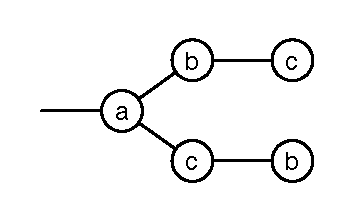
\includegraphics{tree}
    \end{center}
    \vspace{0.43 in}
    \caption{A possible lock tree}
    \label{fig:tree}
  \end{minipage}
  \hfill
  \begin{minipage}[t]{.30\textwidth}
    \vspace{0.26 in}
    \begin{program}
      \FUNCT f(x) \BODY
      \EXP a := 0;
      b := 1;
      c := a;
      \FOR i := 1 \TO x \STEP 1 \DO
      c := a;
      a := b;
      b := b + c;
      \OD 
      a \ENDEXP \ENDFUNCT
    \end{program}
    \vspace{0.26 in}
    \caption{An example program for invariant computation}
    \label{fig:invariants}
  \end{minipage}
  \hfill  
  \begin{minipage}[t]{.30\textwidth}
    \begin{center}
      \begin{small}
\begin{verbatim}
void f() {
  bool {b=a+c},{i<=x};
  {b=a+c} = false;
  {b=a+c} = false;
  {b=a+c} = true;
  {i<=x} = unknown();
  while (*) {
    assume({i<=x});
    {b=a+c} = false;
    {b=a+c} = false;
    {b=a+c} = true;
    {i<=x} = unknown();
  }
  assume(!{i<=x});
}
\end{verbatim}
      \end{small}
    \end{center}
    \caption{An abstraction of Figure~\ref{fig:invariants} using the predicates $b=a+c$, $i \leq x$}
    \label{fig:bebop}
  \end{minipage}
  \hfill
\end{figure*}

Now, the program may evade these problems, but these areas should
still merit some attention.  Accordingly, the threads causing the
warnings and the transitive closure of any thread that writes to any
object read by these threads is generated and called the race window.
The model checker is run on the program with the proviso that only
threads from the race window will be scheduled.  Then the model
checker will be able to determine whether or not this is a real issue,
and yet not have to consider the possibly enormous state space of the
full program.

As an example the authors use the Remote Agent, which is a spacecraft
controller program.  To test their assumptions, they create a large
number of threads that don't change anything the race or modify
threads depend on.  These 40 threads have 10,000 possible internal
states and represent a tremendously large number of possible
executions, so actually running them would take forever.  The authors
then run JPF in simulation mode (that is, with no back tracking) with
the runtime algorithms.  After that, they run JPF in model checking
mode and perform a full exploration of the state space in the race
window.  They find the error immediately and prove it in 25 seconds.

\subsubsection{Dynamically Discovering Program Invariants~\cite{302467}}

The approach here is that while invariants are useful (for automated
analysis, for ensuring that the software still works, and as
documentation) programmers generally don't write them.  The authors
propose a way to automatically detect them.  They repeatedly run the
program in question on different sorts of data and analyze which
invariants, if any, they support.  This is a dynamic analysis, with
all the usual problems like sensitivity to the test runs; if the test
cases are not representative of the input the invariants may be wrong.

The tool to do this instruments the source program to trace variables
of interest, then runs the program repeatedly, and finally checks to
see which invariants out of a library of patterns are satisfied by the
data collected.  The authors' prototype instruments procedure entry,
exit and loop heads; at each point the instrumented code will write
all variables in scope.  After execution, for each instrumentation
point a list of sets of values, one per instrumented variable, has
been collected.  Also, a Boolean variable checking the initialization
state of each variable at each state is collected.

To make these inferences statistically valid, each point in the
program must be repeatedly executed.  The authors have found that they
can repurpose preexisting test suites to do this.  Their inference
algorithm doesn't yet check everything that they want, but it has been
useful for some real world code.  It checks whether any of the
following potential invariants hold throughout the execution:
\begin{itemize}
\item whether any variable is equal to any constant or small number of
  constants;
\item whether a numeric variable is in a given range;
\item whether modulus ($x = a \pmod b$) and nonmodulus ($x \neq a
  \pmod b$) operations on numeric variables hold;
\item whether linear relationships on several variables ($x = a y + b
  z + c$) hold;
\item whether any relationships with all functions in the standard
  library (like \texttt{abs} and \texttt{max}) hold;
\item whether comparisons like $x < y$ hold;
\item any potential invariants over $x + y$ or $x - y$;
\item for sequence variables, whether they are sorted or whether any
  potential invariants over all elements hold;
\item for multiple sequences, whether one is a subsequence of the
  other, or a lexicographic comparison holds;
\item for any sequence and a scalar, whether the one contains the other;
\end{itemize}
and also some negative invariants---things that might have happened
but didn't.  Since this last category is infinite in size, the tool
limits itself to statistically valid conclusions.  As a simplifying
measure for determining whether a conclusion is statistically valid,
the tool always assumes a uniform distribution of values.

There are several important classes of expressions that do not occur
as variables in the source program but are still important; like
$a[i]$ for array indexing.  Accordingly the algorithm introduces
derived variables that are also put through the invariant checking.
Many potential derived variables are uninteresting (for example $x^y$)
and the authors avoid those; they also have measures in place to avoid
introducing arbitrarily many new variables.  Potential derived
variables include
\begin{itemize}
\item the first and last elements and length of any array;
\item the sum, min and max of a numeric array;
\item the element at an index, the subarray up to an index, and the
  subarray beyond an index for an array and a scalar;
\item and the number of calls to the function so far.
\end{itemize}

There are some optimizations needed to make this useful.  For example,
the tool avoids reporting guaranteed relationships like $A[0] \in A$,
and if two variables are equal, it will mark one as canonical and one
as non-canonical.  It will never derive from or further analyze the
non-canonical variable unless the equality is violated.

As an example, consider running the program in
Figure~\ref{fig:invariants} with every integer from 1 to 100.  This is
a simple Fibonacci number generator with a strange extra variable.
The program will not fail to note that the argument $x$ satisfies $1
\leq x \leq 100$ even though this is an artifact of the test set, and
it may conclude that $x \neq 0$ is important.  Similarly, $1 \leq i
\leq x$ will not go unnoticed.  It is not going to discover the closed
form for the Fibonacci function.  It will note that $b = a + c$
throughout the loop head.

\section{Extended Static Analysis}

The goal for static analysis is to prove properties about a program
without running it.  In this manner, one can examine all possible runs
instead of just the one that happened to be selected by the test cases
used.  Doing this right is hard; almost all analyses overstate the
perceived problem and produce false alarms or don't warn on legitimate
issues.

One of the most widespread static analyses these days is the type
system embedded in modern languages.  Type systems are frequently
somewhat limited due to demands that the system be compiled very
quickly, and also due to a desire to be less of an impediment to
making programs work.  I consider only static analyses that go beyond
these limitations.

Static analyses typically have superlinear run times and as a result
don't always scale well to large problems.  As a result of this, many
of the early analyses are restricted to doing intraprocedural
analysis.

\subsection{Extended Static Checking for Java~\cite{512558}}

The goal for the ESC/Java project was a modular reasoning tool about
Java programs that goes beyond type checking.  ESC/Java uses a
automated theorem prover to decide properties of Java methods.  It is
neither sound nor complete; that is, it will not catch every possible
error and it will trigger false alarms.  Rather than try to make
automated theorem proving scale, the authors have opted to perform
only analyses that can be performed in a modular fashion.  They claim
that any tool that does not do this will not scale.

ESC/Java attempts to prove more ambitious things than previous
projects, including presence of null dereferences, array bounds
violations, type cast problems, and also some possible synchronization
errors.  To do this, it is dependent upon annotations.  The tool can
run without annotations, but as \cite{rutar04comparison}~in a
comparison of Java bug finding tools discovered, ESC/Java emits a
large number of warnings in that case.  The comparison in that paper
found that it generated some 12,000 errors on a 3D modeling program,
or 6400 on a BattleTech game.

Most of these annotations were (probably) spurious null pointer
dereference warnings; this occurs because ESC/Java assumes, in the
absence of annotations to the contrary, that any variable can be null
at the start of a method.  The authors claim that between 40 and 100
annotations are required per thousand lines of code in their
experience.  This is expensive to perform on large programs, and as a
result some inference techniques are being investigated.

ESC/Java's annotation language is very similar to the JML modeling
language.  Most annotations are attributes of variables (for example,
that the contents are never null), or are Design By Contract related:
preconditions, postconditions and object invariants.  ESC/Java
supports what it calls ``ghost fields'', which are fields that are
visible to the checker, but not to the Java compiler.  These are
useful for, among other things, making specifications of an abstract
class or an interface more precise without constraining the
implementation.  One difference from JML comes in the specification of
a method in the presence of implementing interfaces.  Since JML and
ESC/Java both permit specifications in interfaces, it is possible that
a Java method may have many preconditions that may interact in a
complicated manner.  JML handles this using a lattice based algorithm,
which is sound; ESC/Java simply takes the union of them all, which is
not sound.

The analyzer is organized into a pipeline: a front end parses the
annotated Java program and converts it to abstract syntax trees, which
are then translated into a language based on Dijkstra's guarded
commands~\cite{dijkstra76discipline}.  To make the problem more
tractable several steps, which can cause the translation to be
incomplete and unsound, are taken.

The first step is related to the modular checking.  When the tool is
analyzing a method and a call to a new method arises, ESC/Java will
use the new method's specification rather than doing any kind of
interprocedural analysis.  The second step is that arithmetic overflow
is not modeled because it causes a tremendous number of spurious
warnings (for example, the theorem prover will repeatedly note that
adding two positive integers can yield a negative one).  The third
step is loops; rather than attempt to compute loop invariants the tool
simply unrolls the loop a number of times.  By default, ESC/Java
unrolls a loop one and a half times, where the extra half is an extra
check of loop condition.

The next step in the pipeline, after the translation, is creating a
predicate that describes all program states where the guarded command
cannot fail.  This is not unlike weakest precondition computations.
Finally, the theorem prover is called on these predicates, and its
output is massaged so that failures in proving get translated to a
complaint about specific lines of code with specific error messages.
A good deal of work has gone into making the theorem prover easier to
post process for this, including the generation of counterexamples.

An additional source of incompleteness present here is that first
order predicate calculus is not completely decidable; as such, the
theorem prover is allowed, after a while, to stop trying to disprove a
purported counterexample.

\subsection{Bug Finding}

ESC/Java is among the most ambitious static checkers, but it is not
the only path that can be trodden.  There exist other less ambitious
checkers that explore similar properties but concentrate on bug
finding, not proving correctness.

\subsubsection{Finding Bugs is Easy~\cite{hovemeyer04finding}}

This paper focuses on developing tools that try to find bugs, not
tools that perform complicated analyses.  The authors look for ``bug
patterns,'' which is code that is deemed likely to be an error.  This
appears to be very useful in practice, as this approach has found
embarrassing bugs in widely used applications and libraries.

The authors' technique is entirely automated and not reliant on test
data.  While formal proofs are of course the ``best'' static
technique, they are so difficult to apply that in practice they aren't
very useful.  Partial verification has enjoyed some success but
defining useful partial verification algorithms is hard.  Instead, the
authors investigate unsound techniques to catch simple problems, with
a watchful eye on the state of false alarms.

These bug pattern detectors use several strategies: some only scan the
class structure and its inheritance hierarchy, some perform a linear
code scan, others are flow sensitive using a control flow graph, and
finally a few perform dataflow analysis.  None of these techniques are
more sophisticated than might be present in an undergraduate level
compiler course.  The dataflow analysis is the most complicated, but
the authors have written a framework to make it easier.  Most
detectors are about 100 lines of code, with the most complex being
1000 including whitespace and comments.

A selection of some of the most interesting detectors used include:
\begin{itemize}
\item checking that \texttt{clone()} is implemented correctly---to get
  the subclass's type correct, the method must call
  \texttt{super.clone ()}, not use \texttt{new};
\item covariant \texttt{equals ()} methods---due to Java's overloading
  semantics, methods like \texttt{public} \texttt{boolean}
  \texttt{equals} \texttt{(Foo obj)} do not override the superclass's
  \texttt{equals ()} method, but because it looks right it can be hard
  to notice this for a problem;
\item ensuring that classes that redefine \texttt{equals ()} redefine
  \texttt{hashCode ()} as well, and vica versa---this is a requirement
  imposed by the Java language, but frequently isn't detected until
  inserting the object into a Hashtable fails mysteriously;
\item letting static fields be modifiable by untrusted code---for
  example, a static non-final field that is public or protected, or
  that references mutable structure;
\item null pointer dereferences, using an intraprocedural dataflow
  analysis.
\end{itemize}

The authors ran these detectors on several widely used programs.  The
detectors run reasonably fast, and largely met the target of 50\% of
reported bugs being real.  Some of these detectors would be good
candidates for warnings in a Java compiler.

So why does this work?  Part of this is comes from the way the Java
language is defined; there are a number of conditions imposed upon
classes that are not checked by the compiler but will cause runtime
errors (for example, the issue with \texttt{hashCode()} and
\texttt{equals()}, or the fact that the requirements for a class to be
serializable are not checked by the compiler).  Also, everyone makes
silly mistakes sometimes---the authors caught several null pointer
bugs where \verb/&&/ was used when \verb/||/ was meant---and
frequently programmers performing maintenance may have an incomplete
idea of how the class should work.

As an aside, the \texttt{hashCode ()} and \texttt{equals ()} confusion
also exists in the Smalltalk language, with the same inexplicable
failures resulting if you don't redefine both of them together.  C++
has something similar, where the rule was that classes that need
virtual destructors also need copy constructors and a specialized
\texttt{operator =}.

\subsubsection{LCLint~\cite{195297}}

This paper describes LCLint, which is an C based tool inspired by the
older C program checker lint.  Much of what lint did was apply some
static type checking to C, which had a notoriously weak type system
pre-ANSI standard and still does in many respects.  Similarly, the
version of LCLint described in this paper spends a lot of time
enforcing a sort of modularity control that we take for granted
programming in more modern languages.  LCLint has been extended
several times to support different types of analyses.

The authors intended to write a more powerful lint, but claim that
this is not really possible without requiring annotations or forcing
certain stylistic decisions.  Their analysis is done on a procedure
level with no real interprocedural analysis done, for the same reasons
ESC/Java chose.

To support a more modular style onto the C language, it has many
warnings for violating abstraction boundaries, like failure to
distinguish between private and public functions/variables/types,
direct access to an abstract type, etc.  LCLint can also check for
undocumented use of globals, undocumented modification of visible
state in a module, and missing initializations.

Many warnings described in this paper cover up weaknesses in C---for
example, C's confusion of characters and integers and booleans and
integers.  The authors claim it has been useful on several C programs,
uncovering a memory leak and some abstraction violations in a small
database; it also helped them understand an automated system builder
that they'd never looked at before.  They make the further claim that
it helps evolve C programs, as evidenced by running it on LCLint
itself; there, it caught some type abstraction problems and helped
verify that an abstract type really was.

\subsubsection{Static Detection of Dynamic Memory Errors~\cite{231389}}

This paper describes an extension to LCLint for handling memory
allocation problems.  This makes it a static, intraprocedural tool and
the extensions to LCLint's specification language must reflect that.
These extensions permit defining weak pre and postconditions for
functions, which can be checked statically.  To make their analysis
more feasible the authors assume that any branch can always be taken,
that the memory effects of any loop are the same as running it zero or
one times, and that compile-time unknown indices or pointer offsets
are either all the same element or independent elements.

Since this targets C, we have to talk about a storage model.  The
paper defines an object as a typed region of storage.  Some of these
are allocated and deallocated by the compiler, and others are managed
by the program.  An object has one of three different states:
undefined if it has been freshly allocated and has not been
initialized, defined if it has been initialized, and completely
defined it is defined and if all storage reachable from it is also
defined.  Using undefined storage as an rvalue is marked as anomalous;
here anomalous means ``flagged as a likely error.''  A pointer is a
typed memory address; it is either live or dead, and using a dead
pointer as an rvalue is anomalous.  It is also anomalous to
dereference an allocated pointer that points to undefined storage.

In addition to tracking the above properties, the tool also traces
null propagations, and assigns owners to objects.  Here, ownership
indicates which references external to the method can legitimately
refer to the object.  It is anomalous for an object to have no owners,
and indicates a memory leak.

The extensions to LCLint's specification language can mark several
broad categories: whether a pointer can ever be null, which defaults
to ``no''; constraining instances of a type; constraining use and
values of function arguments and results; use and value of global and
static declarations.  The default assumption is that all parameters to
a function are completely defined, although this can be relaxed.

The core idea behind handling dynamic allocation is that of
obligation-to-release storage.  This is transferred to the initial
reference upon the creation of the storage, and either the object
should be freed before that reference's scope ends, or the obligation
should be transferred to some other reference.  The obligation can be
transferred to the return value, to a parameter, or to an external
reference.

The extension also tracks aliasing through the ``only'' specification;
any ``only'' reference is supposed to be the only pointer to that
block of storage, and any unexpected aliasing should be highlighted.

The motivation for developing this tool is the memory management of
LCLint itself, which initially used a garbage collector.  This made it
very difficult to port to different platforms, and the code base
resisted several attempts to convert it to manual memory management.
The above techniques helped support the final, successful attempt to
convert LCLint to manual management, and uncovered several weaknesses.
LCLint does some strange memory management in error handling code that
the tool couldn't figure out but which was deemed to be fine.  There
were several places where the alias analysis wasn't sufficient.  The
authors tested the program with explicit deallocation after; this
highlighted some weaknesses in the above techniques that were then
fixed.  Subsequently they tried again and found some storage leakage
from global or static variables.  Ultimately the authors concluded
that doing a static analysis of dynamic memory allocation properly was
impossible without interprocedural analysis, but that this version,
though flawed, was still useful.

\subsubsection{Testing Static Analysis Tools~\cite{zitser04testing}}

This paper attempted to test the usefulness of some static analysis
tools using security vulnerabilities in several Internet daemons
published by CERT.  The authors believed that static analysis tools
were necessary because the dynamic analysis tools available
(StackGuard and the like) tend to turn a vulnerability into a denial
of service attack.

There are a lot of tools for this, but the detection rate is unknown
and the false alarms are hard to assess.  The authors' major goal was
to compute the probability that the static analysis tool in question
would correctly understand the difference between safe and unsafe
versions of the same code.  They examined five tools, one of which is
an extension of LCLint.  The original goal was to run each of them on
BIND, WU-FTPD and Sendmail.  The 14 most recent severe vulnerabilities
would denote bugs that the programs should find.

Unfortunately none of the tools could check all of the code in
Sendmail; the authors did not check BIND and WU-FTPD but presumed that
the experience would be similar.  To avoid this, the authors created
self contained model programs, 90 and 800 lines in length, by
extracting the vulnerable code.  For each of the 14 vulnerabilities,
the authors produced a vulnerable model program and a corrected model
program (according to the maintainer's patch).

The ``corrected'' programs may still have bugs, but they don't have
the bug that caused the CERT notice.  The analysis concentrated on the
lines of code causing the CERT vulnerabilities; to summarize it,
PolySpace C and the LCLint derivative Splint found 87\% and 57\% of
the vulnerabilities respectively while the other three tools found
nearly none.  Both those tools also had high false alarm
probabilities, near 50\% for the lines analyzed.  The authors
concluded that Splint's ability to detect security bugs was not
significantly different, at the 5\% confidence level, from a tool that
marked 43\% of lines in a program as being bad.  PolySpace's detection
abilities were deemed to be statistically significant on the 5\%
confidence level from a randomized tool.

There were a tremendous number of alarms throughout the rest of the
code, PolySpace generating one for every 12 lines of code and Splint
one for every 46.  Some of these may be genuine issues, but the model
programs are too complicated to make that easy to determine.  Instead,
the authors created additional model programs that securely performed
some complicated indirections that were present in the original model
programs and in the daemons themselves.  Splint and PolySpace were
then run on these new programs to check whether the tools reported
false alarms.  Of these two additional programs, one tripped up Splint
and both tripped up PolySpace C.

This is a disappointing performance, and implies that static analysis
programs, to be useful for this important task, will have to get
better at some of the strange things that real world C programs do.
In particular many of the CERT vulnerabilities were not localized to
one function.

\subsection{Algorithms}

All the papers previously discussed deal with tools.  In this section
a pair of algorithms for performing static analysis for verification
are examined.

\subsubsection{Path-sensitive Program Verification~\cite{512538}}

In this paper, the goal is to perform a partial program verification
in polynomial time.  The main idea is that given a temporal state
property encoded in a finite state machine, the analysis tool can
track that state throughout the program.  If an error state in the FSM
is never reached, then the program obeys the property in question.

Obviously, branch correlations are incredibly important for this to be
useful.  Tracking branch correlations usually leads to an exponential
state space.  The proposed algorithm notes that most branches are
probably irrelevant; accordingly, for ``property simulation'' a branch
is relevant only if the FSM transitions to different states along the
two arms of the branch.  If at any merge point in the control flow
graph two states that are being tracked occupy the same position in
the FSM, then they will be merged.  Otherwise they must be processed
independently.

The algorithm given is actually a framework for interprocedural
property simulation; to achieve their polynomial bounds, the authors
focus on the case where the execution states form a constant
propagation lattice.  In this case, the analysis can be done in
polynomial time and space.  The authors have written a tool called ESP
which uses a combination of alias analysis and this simulation to
verify large code bases.  The authors tout their ability to guarantee
that the \texttt{FILE *} argument for \texttt{fprintf} is valid and
open at the time of the call throughout the front end of gcc.

To describe the algorithm, first define a symbolic state is the pair
of a property state, which is a set of states in the FSM, and an
execution state, representing the state of the program at that point.
The analysis uses a theorem prover to determine which paths of a
branch are feasible given the information in the execution state.  At
any merge point, the symbolic states are grouped according to the
property state.  For example, a merge point representing four branches
where one has property state $\{a\}$ and execution state $l$, another
has property state $\{a\}$, and execution state $m$, and so on will be
merged thus:
\begin{multline*}
\alpha \Bigl(\Bigl\{\bigl[\{a\}, l\bigr], \bigl[\{a\}, m\bigr],
 \bigl[\{b\}, n\bigr], \bigl[\{b\}, o\bigr]\Bigr\}\Bigr) = \\
\Bigl\{\bigl[\{a\}, l \sqcup m\bigr], \bigl[\{b\}, n \sqcup o\bigr]\Bigr\}
\end{multline*}

The authors show that the run time for their algorithm is $O(H | E | |
D | (T + J + Q))$, where $H$ is the height of the execution state
lattice, $E$ is the number of edges in the CFG, $D$ is the number of
states in the FSM, $T$ is the cost of theorem prover calls, $J$ is the
cost of joins, and $Q$ is the cost of equality.  In the specific case
of constant propagation, the complexity becomes $O(V^2|E||D|)$ where
$V$ is the number of variables.

The above focuses on a single procedure, but by using a technique
called summary edges in the manner of Reps, Horowitz and Sagiv
in~\cite{reps95precise}---which tries to perform procedure analyses at
most once per independent input context---interprocedural analysis is
feasible.

\subsubsection{Scalable Context-sensitive Flow Analysis~\cite{349332}}

Here, the authors present a way of performing a context-sensitive,
flow-insensitive flow of values analysis.  As a demonstration of the
framework, they present a context-sensitive flow-insensitive points-to
analysis for higher order languages.  The insight here is that
standard Hindley-Milner type inference can be used to capture some
sorts of inter-procedural value dependencies.  Those dependencies can
then be encoded into a type instantiation graph (TIG).  If two nodes
are reachable in the TIG, then values flow from one to the other.  The
algorithm works on higher order programs directly, can answer
points-to queries in time linear in the size of the TIG, and possesses
some other attractive qualities.

An example may be the best explanation of the algorithm.  Consider the
following program:
\NumberProgramstrue
\begin{program}
  \FUNCT f(p_1) \BODY \label{prog:f}
  \EXP |return| p_2() \ENDEXP \ENDFUNCT
  \FUNCT h() \BODY \label{prog:h}
  \EXP |local| \, \tab {} d_3, j_4 := f_5 \, |in|
  j_6(d_7) \untab \ENDEXP \ENDFUNCT
\end{program}
\NumberProgramsfalse

The flow algorithm will generate the set of constraints
\begin{align*}
  \alpha_f & = (\tau_1) \rightarrow^{\ref{prog:f}} \alpha_{r(f)} &
  \tau_1 & = () \rightarrow^2 \tau_2 \\
  \alpha_{r(f)} & = \tau_2 &
%
  \alpha_h & = () \rightarrow^{\ref{prog:h}} \alpha_{r(h)} \\
  \alpha_f & \leq^{5}_+ \beta_3 &
  \tau_3 & = \beta_3 \\
  \tau_3 & = (\tau_5) \rightarrow^6 \tau_4 &
  \alpha_{r(h)} & = \tau_4
\end{align*}
and then solve them, getting
\begin{align*}
  \alpha_h & = () \rightarrow^{\ref{prog:h}} \tau_4 \\
  (() \rightarrow^2 \tau_2) \rightarrow^{\ref{prog:f}} \tau_2 & 
  \leq^{5}_+ (\tau_5) \rightarrow^6 \tau_4
\end{align*}
The substitution $\tau_5 = () \rightarrow \tau_4$ for the
instantiation satisfies the instantiation requirement.  The resulting
TIG is shown in Figure~\ref{fig:tig}.

\begin{figure*}
  \begin{center}
    \leavevmode
    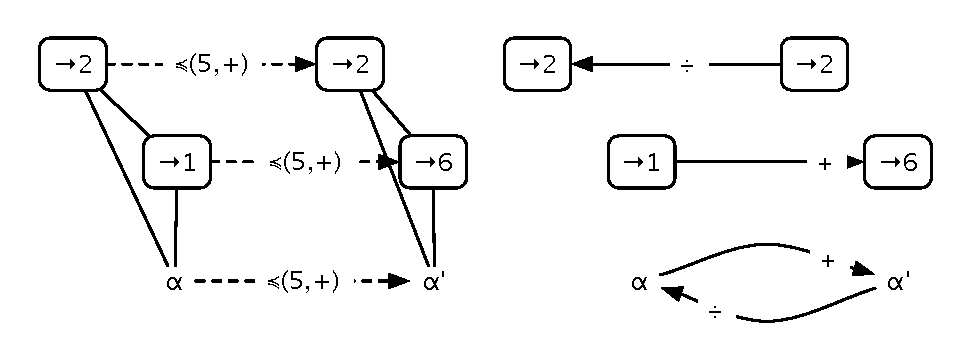
\includegraphics{flow}
  \end{center}
  \caption{Type inference graph and flow graph of example}
  \label{fig:tig}
\end{figure*}

\subsection{Other}

Finally, there are some additional approaches to static analysis that
are interesting enough to mention, and that are grouped together here.

\subsubsection{Typestates~\cite{DBLP:conf/ecoop/2004}}

The core idea is that a normal type system is not strong enough to
express important things about objects.  It is too ambitious to hope
that pre and post conditions might be statically decided, but perhaps
very weak ones could be statically decidable.  For example, the full
state of a stream and the associated pre and postconditions are far
too strong to check.  However perhaps the notion that the stream is
initially closed, is opened by this method, closed by this other
method, and that reading will fail if the stream is not in an open
state, can be checked.

What would be relatively straightforward static analysis is
complicated tremendously by subclassing.  It is important that
subclasses be able to introduce new states, but the subclasses should
not be able to invalidate the analysis of the superclass.  The
mathematics required to handle this is involved, but a high level idea
of what is going on is that the type states of the class combined with
the allowed method transitions give rise to a simple finite state
machine.  Each state of the machine has some simple invariants that
should be true of the object if it is in that state.  It is then the
task of the checker is to verify that each method satisfies the
invariants of the state to which it has transitioned.  The invariants
are kept deliberately simple to make the analysis tractable, and can
include the type states of other classes, some very simple aliasing
concepts, and prohibiting and permitting null values.

The reason that inheritance is awkward is due to the desire to permit
a modular analysis; because we are committed to permitting subclasses
to introduce their own typestates, it is possible for part of the
object to be in one typestate and another part to be in a different
one.  The authors' example uses a caching HTTP client library.  It can
arise that the superclass is in the ``closed'' state, and the subclass
is in the ``cache only'' state.  This means that the user must be
careful about what state the class should be in, and what state its
superclass should be in.

A very simple example of the way this works is the classes in
Figures~\ref{fig:abstract} and~\ref{fig:concrete}.  The challenge here
is that when the union worker starts striking, his superclass believes
he's not working.  For modular analysis to work, the union worker
needs to be careful to maintain that relationship.

\begin{figure*}
  \hfill
  \begin{minipage}[t]{.45\textwidth}
    \begin{center}
      \begin{small}
\begin{verbatim}
[ TypeStates("Working","Off")
class Worker {
  [ Post("Off") ]
  Worker () { ... }
  [ Pre("Off"), Post("Working") ]
  void GoToWork () { ... }
  [ Pre("Working"), Post("Off") ]
  void GoHome () { ... }
  [ Pre("Working") ]
  void DoWork () { ... }
}
\end{verbatim}
      \end{small}
      \caption{A base class using type states}
      \label{fig:abstract}
    \end{center}
  \end{minipage}
  \hfill
  \begin{minipage}[t]{.45\textwidth}
    \begin{center}
      \begin{small}
\begin{verbatim}
[ TypeStates("Striking") ]
class UnionWorker : Worker {
  [ Post("Off") ]
  UnionWorker () : base () { ... }
  [ Pre("Off"), Post("Working") ]
  override void GoToWork () { ... }
  [ Pre("Working"), Post("Off") ]
  override void GoHome () { ... }
  [ Pre("Working"), Post("Striking"),
    Post("Off", Type=Worker) ]
  void Strike () { ... }
  [ Pre("Striking"), Pre("Off", 
    Type=Worker), Post("Working") ]
  void GoBackToWork () { ... }
}
\end{verbatim}
        \caption{A subclass using type states}
        \label{fig:concrete}
      \end{small}
    \end{center}
  \end{minipage}
  \hfill
\end{figure*}

Because this analysis attempts to enforce invariants, it needs to know
about any aliases.  The authors deal with this by allowing the user to
assert that an object is either not aliased, or that it may be aliased
multiple times.  Objects that are not aliased perform normally.
Objects that may be aliased multiple times are not permitted to change
type states except through a technique the authors do not describe.

\subsubsection{Automated Environment Generation~\cite{tkachuk03automated}}

This paper describes a static analysis to create an environment in
which the code being analyzed will run.  This problem is of tremendous
importance for model checking real programs.  The bit of code to be
tested must be exercised in a fashion similar to the way the code that
depends on it will run (what the paper calls the ``environment
assumptions'').  Also, additional code that the target depends on may
be too intricate to simulate perfectly, and it in turn must be
abstracted (what the paper calls the ``environment implementations'').
This can represent a great deal of work.  In~\cite{yang04using} most
of the work involved was in setting up an environment that was
sufficiently convincing that the file system code could run, and yet
not destroy a real disk.

The subject of the paper is the Bandera Environment Generator, which
has two modes of operation for doing this: the first, and the one
described in this paper, is to introduce a language for specifying the
environment that describes everything important.  BEG can also
discover this automatically using the implementing code, although the
authors do not go into great detail about this.

BEG generates among other things a driver which sets up a bunch of
objects to be checked and then exercises the objects.  The
requirements for this driver can be written in the specialized
language and setting up objects is more or less like Java code.
Describing how they should be exercised is done with a sublanguage
that is essentially a regular language on method calls.  For example,
the driver for an \texttt{Iterator} could be expressed as
\texttt{<Iterator i = iterator()>:} \texttt{(i.hasNext();}
\texttt{i.next();} \texttt{i.remove()?)*}.  This expresses the idea
that for any object set up in the driver that has an
\texttt{iterator()} method, that method can be called, its result will
be named \texttt{i}, and then the sequence \texttt{i.hasNext ()},
\texttt{i.next ()}, and possibly \texttt{i.remove ()} will repeat an
arbitrary number of times.

Each exercise specification in this form is translated into Java code,
one thread per assertion.  The model checker itself can be relied upon
to check every possible interleaving of those assertions.

As an example, the above code regarding the Iterator will get
transformed into this Java code, if \verb|x| is the only element in
the environment with an iterator method:
\begin{verbatim}
{
  Iterator i = x.iterator ();
  while (chooseBool ()) {
    i.hasNext ();
    i.next ();
    if (chooseBool ()) { i.remove (); }
  }
}
\end{verbatim}

BEG will additionally produce skeleton code for the required
environment implementations using static analysis techniques; this is
not addressed in any great detail although apparently varying levels
of precision are available.

This area is a highly important area for program checking and relates
to the work I did during an internship with Fujitsu.

\subsubsection{Exploiting Purity for Atomicity~\cite{1007543}}

This paper is related to the atomic analysis described
in~\cite{964023} and~\cite{wang03runtimeRV}.  The main concept is that
since reducibility is useful but isn't powerful enough, it should be
extended.  The manner in which the authors choose to extend it is
through using so-called ``pure'' blocks.  The authors use this to
verify that alleged atomic code is really atomic through a static
analysis.

For the purposes of this paper, a pure block is a block of code whose
normal execution doesn't change the program (and so can, therefore, be
entirely omitted during reduction analysis).  Only if it terminates
exceptionally (using a \texttt{break}, in the framework given) may the
block change the state of the program.  Now, in any interleaved
execution, any pure block that does not terminate exceptionally is
changed to a skip, and the rest can be treated using the normal
reduction semantics.  The proposed algorithm also supports ``unstable
variables'', which are variables that are deliberately not protected
by locks; an example is a packet counter used entirely for statistical
purposes in a networking program, where it is not important that the
counter necessarily be exactly correct.

To decide the atomicity of a statement, the authors use an effect
system (much like a type system but concentrating on the
computations).  This analysis takes place after race condition,
control flow and side effect analysis have been completed.  The code
in Figure~\ref{fig:atomicsuccess}'s deposit method would get verified
as follows: the acquiring of the lock is a primitive that is a right
mover; the read of balance, since its lock is held, is a both mover
with no exceptional behavior; the assignment is a both mover since its
lock is held; the lock release is a primitive that is a left mover;
and since $R ; B ; B ; L = A$ and there is no exceptional behavior
possible, the method is atomic.

The authors apply their framework to some simple code.  The amended
analysis can determine that some cache lookups are atomic, or that
some wait-and-notify loops are atomic.  To make certain styles of
long-running computation optimizations workable, the authors add the
idea of a weakly pure block.  This is like a pure block but that only
changes thread-local variables.

\section{Model Checking Software}

An explicit state model checker is a program that systematically
explores the state space of a specialized almost-program called the
model.  By doing this, absolutely precise statements can be made about
the model at any point in its execution.  There are other approaches
but the explicit state model is the most immediately relevant one for
program checking.  Model checking as a technique excels at checking
complex interactions between a small number of components.  Larger
numbers of components are feasible in theory, but almost every
relevant algorithm is NP-complete.  Ordinary use of model checking
checks only a specification, not a real program.

However, relatively recently there has been a great deal of interest
in the idea of model checking actual programs.  In this way, if the
program doesn't implement the specification correctly it can be
caught.  This also combines the attractive qualities of dynamic
analysis with its precision, and static analysis with its code
coverage into one unified tool.

The biggest problem that program checking runs into is that after the
environment has been generated, the algorithms used are still
NP-complete, and this manifests itself as an exponentially growing
state space.  Different program checkers have different ways of
handling this, but the most successful techniques are still to limit
the scope of the analysis.

Java PathFinder will be considered first, because it is very complete
and useful and will give a framework to discuss other model checkers.

\subsection{Java PathFinder\cite{786967}}

Java PathFinder is a specialized model checker for checking Java byte
code.  As mentioned, this is a something of a remarkable thing.  JPF
has had to address the question ``so why check programs?''  State
spaces are more enormous than normal, programs can be difficult to
formalize and bugs are frequently easier to catch using specialized
tools for the purpose.  Instead, this line of argument goes, one
should model check the design, because that is probably more tractable
and will permit catching errors earlier.

The problem with this approach is that the translation of the design
into real code is not a mechanical process.  Many bugs that are
introduced are not actually design errors; NASA's Remote Agent system
contained several mistakes on the implementation level, one of which
caused a deadlock 60,000 miles into space.  As well, this manner of
development is not necessarily a good way to write programs; it
ignores the importance of iterative development.  The most interesting
reason to verify real programs, though, is because it's hard, and the
problem may drive research into new and interesting places.

JPF's architecture is determined by the task.  The original version of
JPF translated Java code into Promela, the input language for the
model checker SPIN.  This has problems in that the source frequently
needs to be available (although translation of raw Java byte codes is
feasible) and also the target language needs to be able to express the
concepts in the source language.  Since Promela lacked any concept of
floating point numbers, JPF was unable to deal with them.

JPF now uses a custom model checker based on a custom JVM.  It is an
explicit state model checker.  Due to concerns regarding liveness
properties, JPF searches the state space in a depth first manner, but
also can use other search algorithms.

JPF supports all of the Java byte codes, and so every pure Java
program can be analyzed.  Many Java programs escape from the pure Java
environment to the outside world for input and output; things like
accessing the filesystem, network communication, GUIs all require
additional capabilities.  Fortunately many of these escapes can be
simulated with simple wrappers.  Additionally, JPF requires that the
environment a system will execute in be present as well as the system
itself.  This is like testing.  JPF can currently check for deadlocks,
invariants, user defined assertions and LTL formulas.

After the decision to construct a custom model checker had been made,
the next issue became how to deal with states.  To ensure termination,
explicit state model checkers need to store the states that have been
visited; otherwise, loops in the state space that occur will result in
loops in the program (although it should be noted that stateless model
checking does exist, and will be discussed in the paper on
Verisoft~\cite{263717}).  To make storing states work, they need to
take up very little memory, hash quickly, and be comparable
quickly---to underscore this, the entire state of the program, heap,
stack and all must be stored compactly, hash quickly, and be
comparable quickly.  Since JPF has a custom JVM, getting access to
these states easy, but a JVM state is a heavyweight thing.  The
approach taken is to store each component of the state separately in
tables.  The ``JVM state'' is then a collection of indices into these
tables, and when the state changes, the unchanged portions don't have
to be copied.  To permit collapsing the states needed for
backtracking, an un-collapse operation is also called for.

The last problem that needs to be tackled to check Java code is not a
technical issue with checking programs per se; it is a systematic
problem for all model checkers.  This is the state space explosion
problem.  There are several ways to help contain this.

JPF implements several symmetry reductions, which permit discarding
states that are logically equivalent even though they are not
bit-level equivalent.  Symmetries on a Java level come up in many
places but the authors speak specifically of two: class loading and
the heap.  The first problem notes that in Java, classes are loaded
dynamically as references to them come up.  This means that they can
be loaded in an arbitrary ordering that is essentially identical to
any other arbitrary order, but has a different memory image.  JPF
handles this by associating class names to fixed positions in memory,
so that the first time a class is loaded it gets assigned a position,
and any other time that class gets loaded, it goes into the same
position.

Unfortunately this exact solution doesn't work with the heap.
Instead, JPF uniquely identifies every allocation byte code.  That
identifier, combined with the number of times the byte code has been
invoked (incremented upon execution, decremented on backtracking), can
then identify that allocation and place it in the same place in memory
regardless of the run order.  This is not totally satisfactory---two
threads might execute the same allocation code and the symmetry
reduction will be missed.  This could be corrected at the cost of
making the symmetry reduction take longer, and the above scheme was
chosen to represent a sort of sweet spot.  An additional complication
is garbage collection---states with and without garbage should be
equivalent---and JPF uses a variant of mark-and-sweep to handle this.

Another technique for curbing the state space explosion problem is to
abstract irrelevant details.  As an example it is probably not
important that a time counter go through its entire range---it may be
sufficient for it to simply exist at all, or to have one of a handful
of values so that it can be distinguished appropriately, but the whole
$2^{32}$ or $2^{64}$ range of the variable is totally unnecessary.

This could be done during the generation of states, or an abstract
program could be generated and that could be checked instead.  The
authors believe that these abstractions generally impact only one or a
small group of classes and so favor generating abstract programs.
They have developed an abstraction tool that takes a Java program
annotated with predicates and generates a different Java program
operating on them.  The Bandera tool has similar techniques.

A concern about doing this is that the abstract version of the
program, however it is generated, will preserve correctness.  However
the new possibilities may trigger errors that did not happen in the
real program.  How to eliminate these is still a research problem, but
a pragmatic solution exists: any path in the abstracted program that
has no nondeterministic choices is a path in the real program.  As an
alternative, since the original program does exist, it could be
interrogated after a potential error trace has been created.  If the
error trace is really a path in the real program, then well and good;
otherwise, go back and try again.

Another approach to the state explosion problem is to use static
analysis to eliminate uninteresting areas of the state space.  The
three techniques the authors have concentrated on are static slicing,
partial evaluation and partial order computation.  Static slicing
takes a program and a criterion and yields a new, smaller, program
that is equivalent to the old one for the criterion in question.
Partial evaluation tries to simplify expressions through constant
propagation to avoid redundant computation.  Partial order computation
identifies statements that can be safely interleaved with other
threads, and so this interleaving doesn't need to be examined.

The final approach to reducing the state explosion problem is runtime
analysis.  This is spoken of in more detail in~\cite{havelund00using}
discusses above, but the idea is that an imprecise runtime analysis
(which scales tremendously well) is first run on the program, and then
anywhere it claims there is a potential problem is investigated in
more detail with the model checker later.

\subsection{Other program checkers}

There are more model checkers on programming languages than just JPF,
and these are a selected few.

\subsubsection{MAGIC~\cite{776863}}

MAGIC checks that C programs satisfy a label transition system, which
is like a state machine with edge labels.  If the user gives a state
machine, then MAGIC will try to check whether or not the program
reflects that.

MAGIC is intended to fit in as the core of an abstract-verify-refine
loop, although the last step in the loop is manual at this time.  This
idea is that model checking of programs can be done in a more
automatic manner by starting with a very simplistic overabstraction of
the program.  This is run through the model checker.  If no error is
found, then the program satisfies the property desired; if an error is
noted, then it is checked against the original program's predicates.
If the error is legitimate, then we terminate; otherwise, refine the
abstraction so it is less simplistic, and try again.  This is not
really an algorithm because it is not guaranteed to terminate,
although it has worked well in practice.

MAGIC performs this analysis by constructing a control flow graph from
the C program, and then attempts to add some recognition of data flow
into it.  It takes a set of predicates and then expands each location
in the original CFG into $2^k$ new states (where $k$ is the number of
predicates).  Any edges present in the original CFG that cannot be
proven to be false using a theorem prover are transferred to the new
version.  If this new state machine implements the original
specification, then the C program implements the state machine;
otherwise, we go back into the abstract-verify-refine loop, changing
the predicate set to refine the abstraction.  The question of whether
the expanded CFG implements the specification is equivalent to asking
if there is a simulation between two LTS, which can be translated into
a problem in SAT.

\subsubsection{Verisoft~\cite{263717}}

Verisoft represents one of the first program checkers.  There are a
number of architectural decisions made that force numerous compromises
in the analysis.  For example, it runs on largely uninstrumented C
code and makes no attempts to store the state of a running program in
that fashion.  The emphasis is on several cooperating C processes
communicating through a small number of channels.

Because Verisoft does not store states, the usual state space
exploration techniques are unavailable.  More modern checkers for C,
like CMC~\cite{musuvathi:osdi:cmc}, will store states and perform much
more like JPF.  Verisoft has problems with revisiting already explored
portions of the state space.  To avoid this, it uses techniques based
on sleep sets and persistent sets, although it still frequently
revisits old states.  Sleep sets and persistent sets are both partial
order methods; they attempt to determine which actions can interleave
safely and then executing only one combination of them.  A persistent
set is a set of states where, no matter what happens in the current
state, as long as it isn't entering the persistent set, no interaction
with the persistent set is possible.

Sleep sets look for transitions that have already been explored.  For
any node expanded by the algorithm, a set of transitions that the
algorithm does not need to explore are updated.  The idea here is that
if a transition $\alpha$ has already been explored from a state, then
when exploring any other transition that is independent of $\alpha$,
there is no need to explore the $\alpha$ transition from the new set.

\subsubsection{CMC~\cite{musuvathi:osdi:cmc}}

CMC is a model checker on C, like the previous two, but unlike
Verisoft it will store states.  It is claimed to make a good fit with
an event driven model, largely due to its dependence upon transitions,
which are atomic steps that the system can perform going from one
state to another.  It does not do the same instruction level
interleaving that JPF can.

The CMC paper makes an interesting claim: most model checking papers
speak about proving properties of programs, but the authors claim that
a model checker is best applied to a program in order to find bugs.

CMC acts as a scheduler between processes of the system being
executed, and is not unlike Verisoft in this manner.  However, CMC
will save and restore full states.  CMC deals with the state explosion
problem by storing all states on the to-visit queue uncompressed, and
stores only a hash for any other state.  This can cause some problems
with hash table conflicts, although the authors dismiss this as a
concern.  To help state caching, CMC will rearrange heap objects for
the purpose of normalizing the heap state, and CMC can ignore parts of
objects that are considered uninteresting.

To deal with the state explosion problem, the authors make another
interesting claim: they claim that the bugs that are the hardest to
find (and thus the most useful targets for model checking) tend to be
complicated interactions among a small number of processes.
Accordingly, checking small state spaces should be fine.

\subsubsection{Checking JML with Bogor~\cite{Robby-etal:TACAS2004}}

This paper describes a program for verifying JML specifications of
Java code, by translating everything to the Bogor model checker.
Bogor is attractive here because JML is very complicated; Bogor is
extensible and has the ability to reason about a dynamic heap.  This
is not the only tool to use JML specifications.  It is not even the
only tool to translate them to another language.

Most of the work is in translation.  The Java notions of method
overriding, inheritance, etc., all need to be translated into the
model checker's language.  Other things that need to be translated are
the combination of preconditions, postconditions and object
invariants.  To handle this last bit, the authors have extended Bogor
to directly represent almost all JML expressions.  These include heap
reachability and the accessing of old objects for use in
postconditions.  This translation also has correctness implications in
that the checking of the conditions are now atomic in the presence of
concurrency.  This is an important consideration for JML because of
the power of JML expressions.  There are also a few constructs in JML
that are tricky to check due to aliasing constraints; being able to
examine the heap makes this easy to deal with.

The authors have only checked the translation on small programs so
far, where it more or less worked.  They have noted that partial order
reduction was tremendously useful, which is in line with the JPF
experiences.

\subsubsection{Bounded Model Checking on C and Verilog~\cite{775928}}

This model checker is unlike the previous ones discussed in that it is
bounded.  The idea is that the authors want to reason about low level
C programs that implement circuits.  To avoid dealing with loops, the
tool simply unrolls them up to N times and then checks that further
executions will not break the properties of interest.  This is not a
general technique but it appears to be very successful in verifying C
programs that are intended to simulate hardware.  Checking general C
programs was not a goal; the goal was to ensure that a (presumably
well tested and debugged) C program that simulates a circuit has the
same behavior as something that is supposed to be that circuit,
written in a language like Verilog.  Here, the C program is used as a
specification for the Verilog chip.

The approach taken is to turn a program and its specification into
Boolean formulas and then feed them to a SAT solver.  To achieve this,
the tool transforms the C program extensively.  First, it turns the C
into a program with finite extent.  Then, the tool converts the program
to two bit-vector equations $C$ and $P$ (representing the constraints
and then the property of interest).  Finally, the tool runs a SAT
solver on $C \wedge \neg P$.

The conversion of most operators in C to this binary form is
straightforward and resembles the construction of arithmetic circuits
in hardware.  Dynamic memory allocation is supported, but it is
implemented using uninterpreted functions.

The idea of turning C programs into something finite that can be
verified easily is not uncommon.  Bebop~\cite{ball00bebop} operates on
Boolean programs, and MAGIC~\cite{776863} translates a C program to a
label transition system and then runs a SAT solver on that.  An
important distinction is that both Bebop and MAGIC use the finite
program as an approximation of the full C program.  This checker
intends the finite program to represent the full C program, and will
not work on general C programs as a result.

\subsubsection{Bebop~\cite{ball00bebop}}

The Bebop model checker is intended to be a part of the
SLAM~\cite{503274} project.  It is designed to be used as part of an
abstract-verify-refine loop with C2BP~\cite{ball01automatic}.  C2BP
abstracts C programs using a set of predicates into Boolean programs
that Bebop operates on.

Unlike checkers like JPF, Bebop is a symbolic checker.  It endeavors
to make a single pass through the program, doing all the work by
combining Boolean formulas with the effects of the paths in question.
The authors claim that Boolean programs are a useful target, since
reachability and termination in Boolean programs is decidable (the
programs are equivalent to push down automatons), but the program
retains the control flow of the original.  Since the Boolean variables
can represent arbitrary predicates, relationships between data and
control can be captured fairly easily.

Bebop's main task is, given a Boolean program $B$ and a statement $s
\in B$, to answer whether $s$ is reachable in $B$, and if so to
produce the shortest trace to it.  To do this the authors have adapted
the interprocedural dataflow analysis of Reps, Horowitz and
Sagiv\cite{reps95precise} which~\cite{512538} also uses.  That is,
upon reaching a call site, the algorithm will compute the summary of
the input/output behavior of a procedure, and then whenever the input
context recurs it will use the summary instead of reanalyzing.  Bebop
uses an explicit control flow graph representation rather than
encoding it with BDDs as other tools choose, because it permits
standard compiler optimizations to the flow graph.

Bebop exploits variable scoping rules, and because of this the time
and space complexity is $O(2^k E)$ where $k$ is the number of
variables in scope at any given point and $E$ is the number of edges
in the control flow graph.  This means that if $k$, which is dependent
on the number of predicates used when this is run as a part of the
SLAM toolkit, can be held down the algorithm will run nearly linearly.

To test the program and its run time, the authors ran it on synthetic
programs from a template set up so that at all times only four
variables were in scope.  These synthetic programs make a tremendous
number of calls to procedures.  The running time turns out to be
superlinear (quadratic, in fact) because of inefficiencies in both BDD
libraries used.  The authors believe that if these inefficiencies are
cleared up, the behavior will be linear.

\subsubsection{BLAST~\cite{henzinger03software}}

The classical abstract-verify-refine loop was referred to in the
MAGIC~\cite{776863} paper.  BLAST attempts to implement this loop, but
to make it quicker by abstracting on the fly.  The idea is that if
there is no path to the error label, then the program is fine;
otherwise, check to see if the error path is feasible right away.  If
it is infeasible, refine right away (that is, in the middle of
checking).  This avoids repetitive work.

BLAST runs on C programs represented as control flow automata, which
are just control flow graphs with operators on the edges.  First, the
tool builds a reachability tree where each node is a vertex of the CFA
and a reachable region formula (initially empty).  The refine step
described above is done by asking a theorem prover to suggest new
predicates.  The tool will then add those predicates to the smallest
subtree containing the error.

This way, only the reachable portion of the tree is abstracted,
permitting different precisions at different parts of the state space.
This in turn means fewer predicates need to be processed, and redoing
acceptable work is avoided.  This technique can discover invariants.

The implementation of the tool runs on a C program and produces either
an error trace or an ELF executable with attached proof of
correctness---or, of course, fails to terminate.  It handles all of C
syntactically, including pointers, structures and procedures, but it
models integer arithmetic as infinite precision and uses a logical
memory (that is, for $p + i$ for some pointer $p$ and integer $i$, it
is assumed that it points to the same object as $p$).  BLAST assumes
that the C program does nothing that changes the layout pattern, that
there are no partially overlapped objects, and that pointer arithmetic
is presumed to respect array bounds, etc.  A further omission is that
the tool doesn't handle recursive functions yet.

To make this process efficient, the bottleneck of calls to the theorem
prover must be reduced.  The authors minimize this in several ways: a
faster successor function that is less precise than it could be, only
invoking the theorem prover on predicates that are affected by the
statement in question, keeping only satisfiable disjuncts for the
predicates, removing any predicates referring to variables that are
not in scope, and performing the state comparison entirely on the
Boolean level without interpreting the predicates.  This means that
the tool runs on several thousand lines of C in a few minutes.

\subsection{Applying Program Checking}

In this section a few papers where model checking is applied to
existing programs are discussed; the first runs parts of the Linux
kernel.

\subsubsection{Finding Serious Filesystem Errors~\cite{yang04using}}

The goal here is to analyze file system implementations in the Linux
kernel and verify that in the event of a crash, the file system will
recover to a correct state.  These are always tricky pieces of code
and are not easy to reason about or test.

The authors choose to use CMC~\cite{musuvathi:osdi:cmc} and applied it
to JFS, ReiserFS and ext3, finding 32 serious bugs (most with patches
within a day of diagnosis), every one of which has events that can
lead to unrecoverable destruction of metadata and entire directories.

There are four parts to the tool: CMC running the Linux kernel, a test
driver, a permutation checker (which verifies that no matter what
order the buffer cache contents are written to disk, it can recover)
and fsck.  The model checker starts with an empty formatted disk and
generates and checks states.  The state transitions are either test
driver operations or FS-specific kernel threads which flush blocks to
disk.

The test driver uses the system call interface to fiddle with the file
system.  In every new state, disk writes are intercepted by using a
virtual block device and forwarded to the permutation checker.  The
permutation checker verifies that the disk is in a state that fsck can
repair.  It does this by running fsck on the host system outside of
the model checker and capturing all its disk accesses.  This structure
permits checking for failures in fsck.

After the permutation and file system checking is done, the model
checker traverses the filesystem and checks that the image is the file
system it was expecting.  If errors are detected the new state is
discarded; otherwise it is stored and put on the state queue for
later exploration.

After each system call, the tool compares the filesystem against what
it believes to be the correct volatile file system.  It calls this
VolatileFS and it reflects all operations done sequentially including
the last one.  After every disk write, it compares the checked
filesystem against what it believes to be the correct stable file
system (StableFS), which reflects what the FS should recover to after
a crash.

A possible weakness with the approach is that the authors have only
checked small disks with just a few nodes.  In response to this
criticism they echo the claim from the CMC paper that model checking
works best on complex interactions of small numbers of objects.

The tool checks for a variety of things.  The only parts that are
filesystem specific are checking that reordering the dirty buffer
cache (as can happen on the hardware level) will still give a
recoverable disk, and also checking that if the machine crashes while
fsck is running they will still get a good filesystem.  Checking this
last data point turned out to be very tricky, mostly because
understanding truly arbitrary buffer reorderings is very hard; to make
these bugs easier to understand and fix, a lot of effort was spent in
trying to force fsck bucks to manifest themselves using only more
understandable types of buffer reorderings.

The above techniques found numerous bugs, including a lot in the fsck
recovery stage.

\subsubsection{Predicate Abstraction of C Programs~\cite{ball01automatic}}

The goal here is to abstract an infinite state space into something
tractable for software model checking.  The authors suggest predicate
abstraction as a promising approach, where concrete states are mapped
to abstract states according to how they satisfy a finite set of
predicates.  At the time, the general task on something like C had not
been demonstrated.

Accordingly the authors present C2BP, which performs automatic
predicate abstraction of C programs.  Given a program $P$ and a set
$E$ of predicates, it generates a Boolean program $BP(P, E)$ which is
an abstraction of P and is suitable for feeding to
Bebop~\cite{ball00bebop}.  The goal is that the Boolean program has
the same control flow structure but contains only $|E|$ boolean
variables.  C2BP guarantees that every feasible execution path in the
C program is feasible in the Boolean program.

C2BP has been applied to pointer manipulating programs to identify
pointer invariants, to get more precise aliasing information and prove
structural properties of the list manipulating too as well.

As an example, consider the Fibonacci program in
Figure~\ref{fig:invariants}.  We will use $b = a + c$ and $i \leq x$
as the predicates to abstract on.  This translates to a Boolean
program as in Figure~\ref{fig:bebop}.  Now we can ask whether $b = a +
c \wedge \neg i \leq x$ is true by the end of the function using
Bebop, getting the answer yes.

This is hard in C for several reasons.  Among them:
\begin{itemize}
\item Assignments through dereferenced pointers.  The authors deal
  with this by putting pointers and pointer dereferences in the
  predicates, and using points-to analysis to improve the precision of
  the abstraction;
\item Procedures.  The authors handle this by permitting procedural
  abstraction in the Boolean program;
\item Procedure calls.  This abstraction is difficult in the presence
  of pointers, but the authors handle pointers soundly and precisely;
\item Unknown values.  Here, it is not always possible to determine
  what a statement will do to the predicates.  The authors handle this
  with nondeterministic control.
\end{itemize}
There are some extensions to the technique that may be desirable.  For
example, it may be the case that two predicates in $E$ cannot
simultaneously be true, and it may be necessary to require that the
Boolean program honor this.

There is also something of a precision-efficiency tradeoff present in
doing this correctly.  To compute the abstraction for each statement
with respect to the predicate set can require a theorem prover, and in
the worst case this can involve $O(2^{|E|})$ calls.  The authors have
several techniques to reduce this number, some of which yield an
equivalent program and others of which trade off precision for speed.

These optimizations are mostly changes like not including bits that
can't change, eliminating redundant predicates, some syntactic
heuristics to avoid the call altogether, and caching all theorem
prover computations.  All of these are harmless to precision, and
while the run time is still exponential the optimizations help most of
the time.  If you're willing to sacrifice precision, you can throw
away conjunctions that are too long, or you could call the theorem
prover on the individual components of conjunctions (which works) and
disjunctions (which can lose precision) rather than the problem as a
whole.

C2BP only handles a single thread of execution at the moment.  To
handle concurrent execution the authors would need an appropriate
notion of atomicity and need to account for cross-thread interference.
An additional complication is that model checking Boolean programs
with two threads of control is undecidable.  The authors also suggest
automated predicate generation as a promising area for future work.

\subsubsection{The Bandera Specification Language~\cite{corbett00language}}

In this paper, the goal is a language for expressing constraints, like
LTL or CTL, but closer to the language being checked and not specific
to the model checker in use.  This last requirement is important
because Bandera targets model checkers that don't have a common
specification language and may not express Java concepts directly.

The proposed language breaks the problem into chunks.  An assertion
sublanguage in the program context names all the various results to be
observed, or assertions to be checked.  A temporal property
sublanguage that uses the above named bits to form propositions that
should be checked.  The language is not based on any particular logic:
instead it uses patterns for expressing concepts, like ``X happens
between Y and Z'' or the like.

The assertion sublanguage is embedded in something like Javadoc.  It
is passed through a preprocessor, which goes through and changes
assertions into executable checks using Bandera.assert (boolean).  The
temporal specification language is a little different, by necessity.
It does not handle assertions directly because those are much more
efficient to check directly than using temporal properties.  The
temporal specification language uses patterns of five basic types:
\begin{itemize}
\item global,
\item after the first occurrence of an event,
\item before the first occurrence of an event,
\item between a pair of events,
\item or during the interval between two events.
\end{itemize}
These patterns are translated to the model language of the model
checker in use, or generate Java.  Generating Java code permits
targeting a model checker like JPF.

\section{My Experiences}

I spent September of 2004 working as an intern for Fujitsu, where I
analyzed some of their software.  I did this primarily using JPF.  I
am yet not permitted, due to an NDA, to speak in great detail about
the software, but I can still make comments that are very relevant.

I was called upon to test a program that was many hundreds of
thousands of lines and that had never had any sort of automated
analysis performed upon it.  There were no annotations, no contracts,
and no hope for writing them in the time allotted.  Despite this I was
successful in finding several errors using JPF, by and large without
running into problems with state space explosion.

I was totally ignorant of the product coming in, and knew only of a
persistent deadlock problem the original programmers were having that
went away when they changed databases.  I felt examining the database
code was a good first course of action.  I examined a part of a
concurrency protocol for access to the database and found a
catastrophic problem.  The code that handled premature disconnection
of clients of the database was wrong.  JPF was invaluable for proving
that this problem was real.  I was able to put the code through its
paces while searching for violations of a fundamental, though somewhat
implicit, system invariant, and since JPF would check all possible
interleavings I did not have to worry about scheduling threads so that
the problem was repeatable.

After this success, I went on to examine a different piece of
concurrent code at the urging of the programmers.  After finding
several problems that a tool like FindBugs
in~\cite{hovemeyer04finding} could have caught, I concluded that the
core of the module was basically okay.  To make sure, I started
putting it through its paces in JPF.  This uncovered a latent
initialization bug that was sufficiently subtle that I was convinced
for a week that my environment was somehow subtly violating the
parameters of the tool---the module was in wide use, after all.

I feel this experience has given me an important perspective on the
application of such techniques to industry.  Specifically, I have
concluded the following: tools like ESC/Java and LCLint, although they
are impressive, are not used because they require too much up front
work.  Something like FindBugs has, I think, a rich future in a market
like this due to its focus on low hanging fruit and its attention to
reducing false alarms.

Concurrency makes tools more attractive.  Concurrent bugs are
frequently so difficult to diagnose and so easy to trigger that tool
support is almost essential.  Some algorithms like Eraser's LockSet or
the GoodLock algorithm are useful in their present state, and indeed
the Eraser paper mentions finding problems in widely run C code with
their techniques.

But now, what use does model checking have?  Surely if ESC/Java
requires too much work, then the amount of effort involved in setting
up a model checker is totally out of the question.  To a large degree,
it is.  I would estimate that 80\% of the time I spent on the Fujitsu
code was spent writing environments, but I think the sheer
thoroughness makes it worthwhile.  It is unlikely that many of the
bugs found in~\cite{yang04using} would have been found without the
comprehensive buffer reordering checks that the paper demanded.

I had another atypical experience in that I did not run into the
problems with state explosion that bedevil most program checkers.  I
believe this might have been for any of three reasons: one is that I
was frequently testing chunks of the code, rather than the entire
program at once; a second potential reason is that the code I was
analyzing frequently did not perform intricate calculations, unlike
the filesystems checked in~\cite{yang04using}; and finally, a lot of
the complexity involved with managing state was moved to the database.
Provided the transactions were correctly set up, the database is
supposed to handle the details of recovery, out of order execution,
and long running transactions, meaning the model checker doesn't have
to.

We do not seem to be at the point where arbitrary programs can be
model checked.  However, we are at the point where some real world
programs have been model checked after an expert in the field spent
some time sorting out the issues.  I believe that the main holdup is
the time spent in environment generation.  If this can be made easier,
then we may be able to make program checking a standard tool for
critical components, rather than an inaccessible novelty.

\end{multicols}

\SBtitlestyle{simple}
\SBsubtitlestyle{none}
\bibliographystyle{abbrv}
\bibliography{mae}

\end{document}

%% arch-tag: 2af902b5-97f4-4133-a3bd-f49a42511bc2
